\begin{figure}[h]
\centering
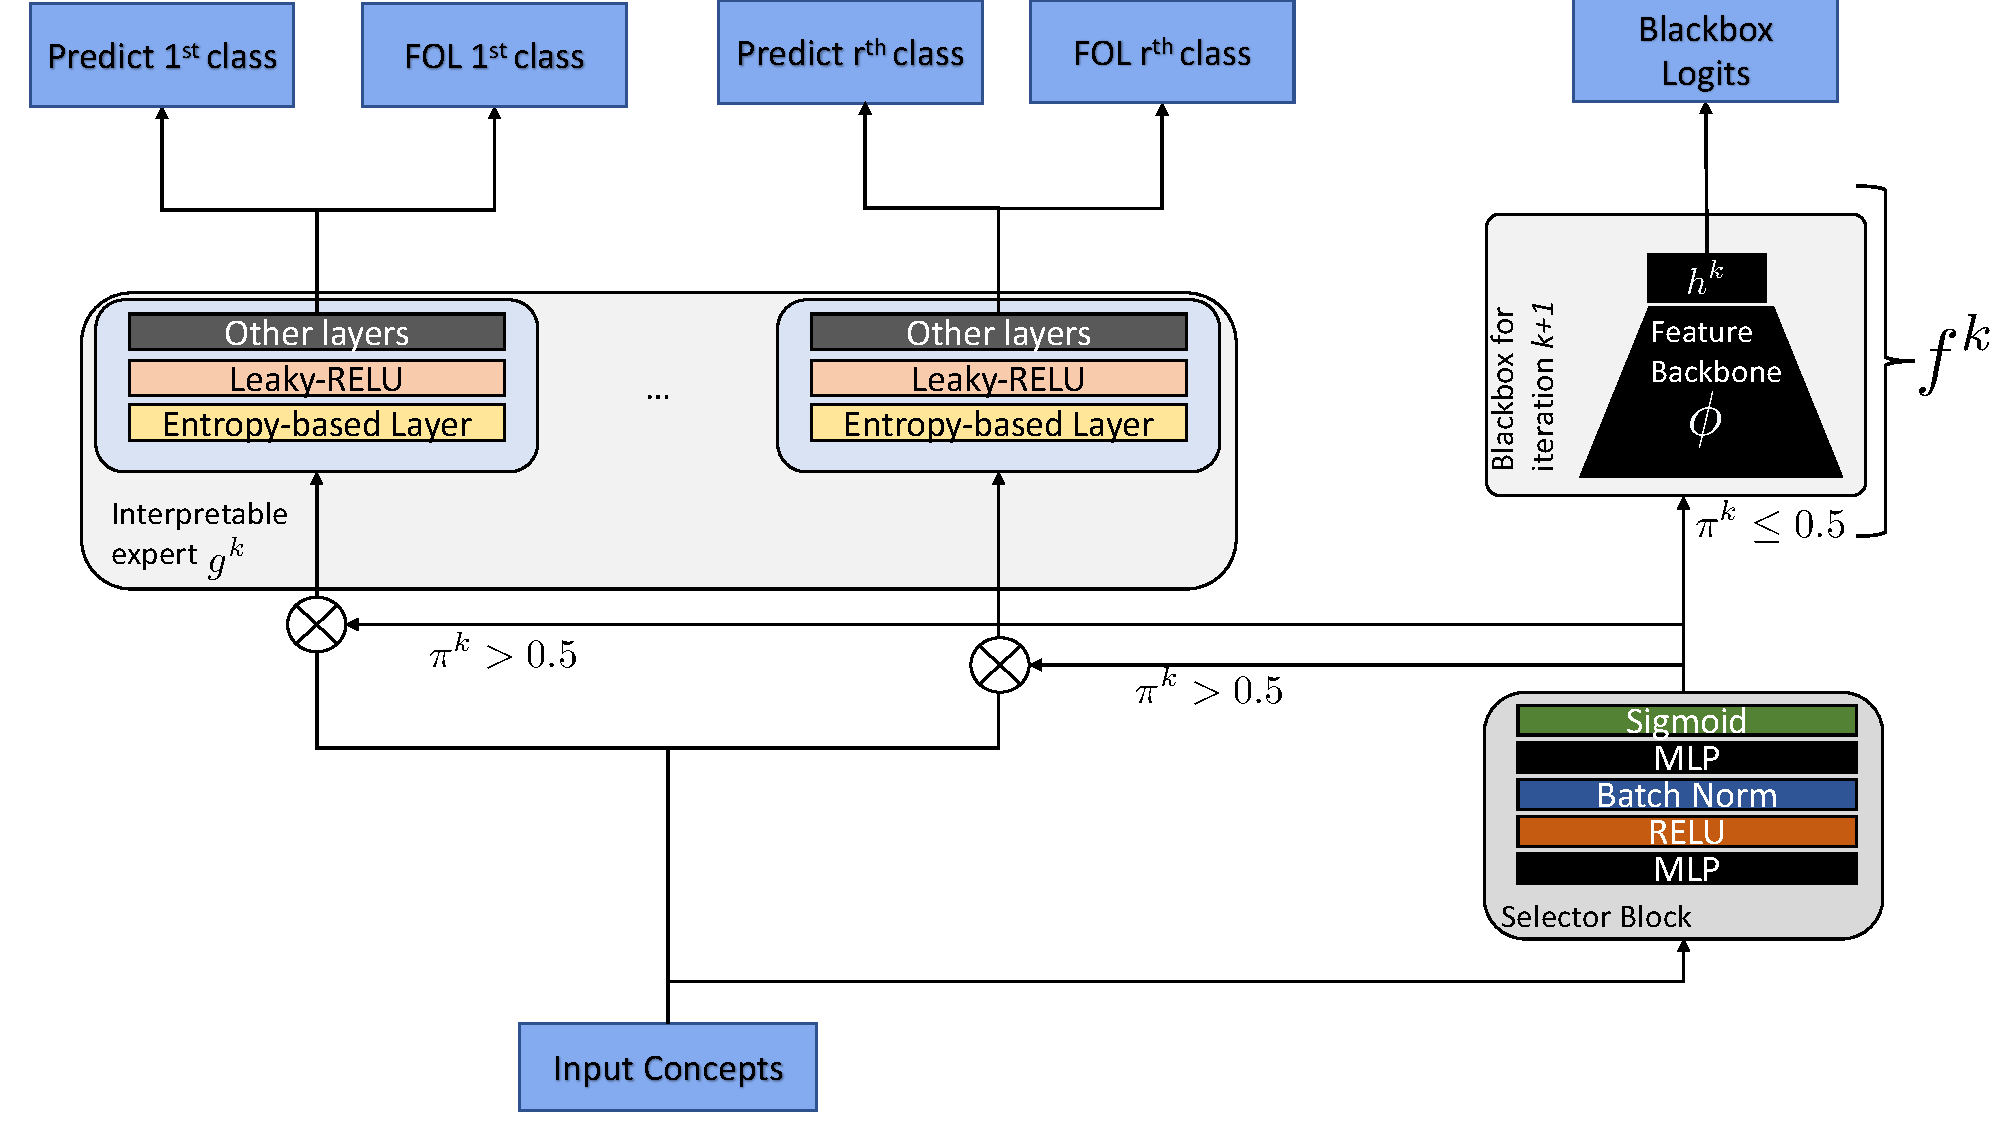
\includegraphics[width=1\textwidth]
{figures/Supp/Architecture.pdf}
\caption{Architecture of MoIE. In an iteration $k$ during inference, the selector routes the samples to go through the interpretable expert $g^k$ if the probability $\pi^k \ge 0.5$. If $\pi^k < 0.5$, the selector routes the samples, through $f^k$, the Blackbox for iteration $k+1$. Note $f^k = h^k(\Phi(.)$ is an approximation of the residual $r^k = f^{k-1} - g^k$.  }
\label{fig:architecture}
\end{figure}

\begin{algorithm}[h]
   \caption{\emph{Route, interpret} and \emph{repeat} algorithm to generate FOL explanations locally.}
   \label{algo: train}
\begin{algorithmic}[1]
   \STATE {\bfseries Input:} Complete tuple: \{$x_j$, $y_j$, $c_j$\}$_{j=1}^n$; initial blackbox $f^0 = h^0(\Phi(.))$; K as the total iterations; Coverages $\tau_1, \dots ,\tau_K$.
   \STATE {\bfseries Output:} Sparse mixture of experts and their selectors $\{g^k, \pi^k\}_{k=1}^K$ and the final residual $f^K = h^K(\Phi(.))$
   \STATE Fix $\Phi$.
   \FOR{\texttt{$k=1 \dots K $}}
       \STATE  Fix $\pi^1 \dots \pi^{k-1}$.
       \STATE Minimize $\mathcal{L}^k$ using equation \ref{equ:final_loss_g} to learn $\pi^k$ and $g^k$.
       \STATE Calculate $r^k = f^{k-1}(.) - g^k(.)$
       \STATE Minimize equation \ref{equ: residual} to learn $f^k(.)$, the new blackbox for the next iteration $k+1$.
       \ENDFOR
        \FOR{\texttt{$k=1 \dots K $}}
            \FOR{sample $j$ in \texttt{test-set}}
                \REPEAT
                    \STATE Initialize \texttt{sub\_select\_concept} = $True$
                    \STATE Initialize the \texttt{percentile\_threshold} = $99$.
                    \STATE Retrieve the predicted class label of sample $j$ from the expert $k$ as: $\hat{y}_j = g^k(c_j)$
                    \STATE Create a mask vector $m_j$. $m_j[i] = 1$ if 
                    $\Tilde{\alpha}[\hat{y}_j][i] \geq$ percentile$(\Tilde{\alpha}[\hat{y}_j]$, \texttt{percentile\_threshold}$)$ and $0$ otherwise. Specifically, the $i^{th}$ entry in $m_j$ is one if the $i^{th}$ value of the attention score $\Tilde{\alpha}[\hat{y}_j]$ is greater than (\texttt{percentile\_attention})$^{th}$ percentile. 
                    \STATE Subselect the concept vector as $\Tilde{c}_j$ as: $\Tilde{c}_j = c_j\odot m_j$
                    \IF{$g^k(\Tilde{c}_j) \neq \hat{y}_j$}
                        \STATE \texttt{percentile\_threshold} = \texttt{percentile\_threshold} - 1
                        \STATE \texttt{sub\_select\_concept} = $false$
                    \ENDIF
                \UNTIL \texttt{sub\_select\_concept} is $True$
                \STATE Using the subselected concept vector $\Tilde{c_j}$, construct the FOL expression of the $j^{th}$ sample as suggested by~\cite{barbiero2022entropy}.
            \ENDFOR
    \ENDFOR
\end{algorithmic}
\end{algorithm}

\cref{algo: train} explains the overall training procedure of our method.~\cref{fig:architecture} displays the architecture of our model in iteration $k$.


% \begin{algorithm}
% 	\caption{Training the MoIE to generate FOL explanations locally.} 
% 	\label{algo: train}
% 	\hspace*{\algorithmicindent} \textbf{Input:}  
%         {
%             Training set: \{$\mathcal{X}$, $\mathcal{Y}$, $\mathcal{S}$\}; trained blackbox $f^0 = h^0(\phi(.))$ using supervision of $\mathcal{Y}$; K as the \# iterations; Coverages $\tau_1, \dots ,\tau_k$
%         } \\
%         \hspace*{\algorithmicindent} \textbf{Output:}  
%         {
%             Sparse mixture of experts and their selectors $\{g^k, \pi^k\}_{k=1}^K$, 
%         }
% 	\begin{algorithmic}[1]
%         \State Fix $\phi$.
%         \State Train $t$ by minimizing BinaryCrossEnt($t(\phi(\boldsymbol{x})$, $\mathcal{S}$)
%         \State Form a concept bank $\mathcal{C}$ with p concepts after discarding the concepts whose validation auroc (accuracy) $\leq$ 0.7 (70\%)
%         \For{\texttt{iteration $k=1 \dots K $}}
%             \State Fix $\pi^1 \dots \pi^{k-1}$.
%             \State Minimize $\mathcal{L}^k$ using equation \ref{equ:final_loss_g} to learn $\pi^k$ and $g^k$.
%             \State Calculate $r^k = f^{k-1}(.) - g^k(.)$
%             \State Minimize equation \ref{equ: residual} to learn $f^k(.)$, the new blackbox for the next iteration $k+1$
%         \EndFor
%         \For{\texttt{experts $k=1 \dots K $}}
%             \For{\texttt{each sample in the test-set}}
%                 \State \label{12}Sort the concepts according to their attention scores from different experts in descending order.
%                 \State Initialise FOL\_bucket as empty list.
%                 \State Select one concept $\{c^i\}_{i=1}^p$ at a time from the sorted concept bank in step \ref{12} until 
%                 \hspace*{\algorithmicindent} \quad $g(c^i$) = g($\boldsymbol{c}$) and add those concepts in the  FOL\_bucket.
%                 \State Construct the FOL expression from FOL\_bucket using \cite{barbiero2022entropy}.
%             \EndFor
%         \EndFor
% 	\end{algorithmic} 
% \end{algorithm}


